% Drawing 154/02-10 -- folder 154, batch 02, archive page 36 (PDF page 37).
% Transcription: figure : un disque au bord vert traversé de cordes orange ; en haut et en bas du bord, deux petits segments bleus où aboutit un faisceau de cordes presque parallèles
% Kind: chord system in a disk. Method 2 (redrawn from the facsimile). Status: partial.
% Notes: A disk with a green rim crossed by eight orange chords, redrawn strand by strand from the 400 dpi facsimile: a bundle of four nearly vertical chords from the short blue arc at the top of the rim (three of them) and from the upper right rim (one, bending down at the top of the bundle) to the short blue arc at the bottom; four transverse chords from the left rim to the right rim. The rim is drawn green with the two blue arcs in place of the gaps where the bundle ends. Pairwise crossings checked: every pair crosses at most once, exactly when its ends interleave on the rim (22 crossings). Still differs from the facsimile / doubtful: the chord from the lower left rim rises to the bundle and then runs along the chord from the left rim, which it crosses at a grazing angle before rising to the right rim (the facsimile shows a single band there; the reading of which end goes with which is doubtful); the short dark scribble on the lower right chord and the yellow ticks inside the rim are left out. Redrawn 2026-11-09 (issue 128): to check again.
% Coordinates: 1 unit = 1 mm = 1/100 of the crop width (bbox in page fractions: [0.143, 0.15, 0.275, 0.243]).
% Redrawn by Claude (claude-opus-5-5), issue #73, 2026-11-07; not checked by a human; not compiled (no TeX in the session).
% Redrawn by Claude (claude-opus-5-5) 2026-11-09 (issue #128, third pass): strands traced one by one on the 400 dpi facsimile (positions read off the colour mask), pairwise crossings checked inside the disk, shared ends computed once, regions bounded by their strands; labels at \small. Not compiled. Status: partial.
% Corrected by Claude (claude-fable-5-2) 2026-11-12 (issue #128, triage on the 400 dpi colour facsimile): seven chords, not eight. The chord from the upper right rim comes down the bundle and leaves it to the lower left rim, crossing the leftmost bundle chord at (39,-72); the chord from the left rim (9,-39) turns up to the right rim (89,-41); its other, short branch to the lower right rim, which carries black cross-strokes, is read as struck and left out. Three bundle chords end on each blue arc. 18 crossings (all pairs except the three bundle chords among themselves). Not compiled. Status: partial.
% Rights: reproduces part of the work -- behind RENDER_TRANSCRIPTS, never published by itself.
\documentclass[tikz,border=3pt]{standalone}
\usepackage{amsmath,amssymb}
\usetikzlibrary{patterns,arrows.meta}
\tikzset{Or/.style={orange!90!black}, Ye/.style={yellow!80!orange}, Lg/.style={green!60!black!70}, Dg/.style={green!45!black}, Br/.style={brown!80!black}, Rd/.style={red!85!black}, Bl/.style={blue!70!black}, Gy/.style={black!40}, pencil/.style={black!45}, struck/.style={black!35}, mark/.style={circle,draw,inner sep=1.3pt}, pt/.style={circle,fill,inner sep=0.9pt}, opt/.style={circle,draw,fill=white,inner sep=1.1pt}}
\colorlet{Or}{orange!90!black}\colorlet{Ye}{yellow!80!orange}\colorlet{Lg}{green!60!black!70}\colorlet{Dg}{green!45!black}\colorlet{Br}{brown!80!black}\colorlet{Rd}{red!85!black}\colorlet{Bl}{blue!70!black}\colorlet{Gy}{black!40}
\begin{document}
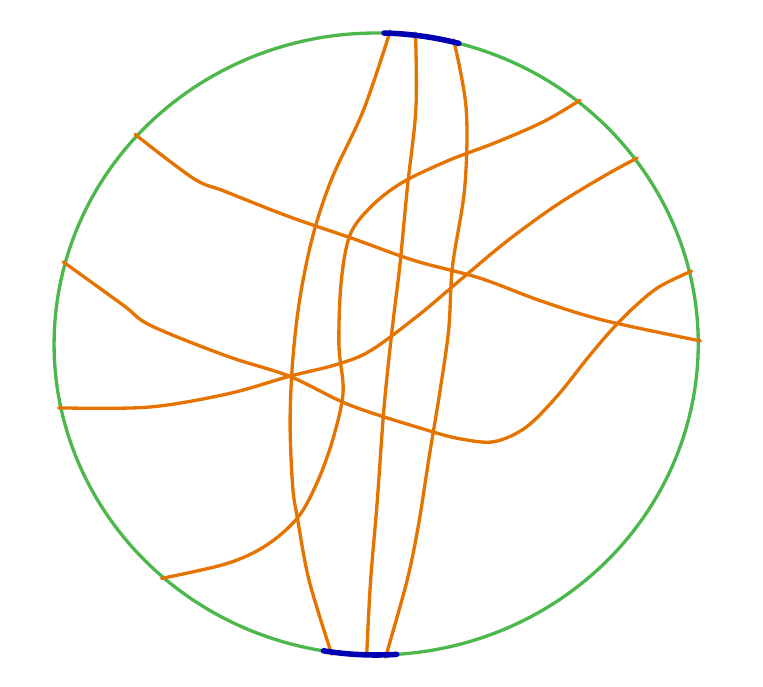
\begin{tikzpicture}[x=1mm,y=1mm,line cap=round,line join=round,font=\scriptsize]
\draw[Lg,very thick] (59.5,-11.72) arc[start angle=75.12, end angle=-86.36, x radius=40.9, y radius=39.5];
\draw[Lg,very thick] (42.3,-88.87) arc[start angle=-99.43, end angle=-271.4, x radius=40.9, y radius=39.5];
\draw[Or,very thick] plot[smooth, tension=0.55] coordinates {(50.79,-10.15) (47.41,-20.15) (43.42,-28.78) (41,-36) (39.33,-44.01) (38.4,-52.02) (38.07,-60) (38.4,-68) (39,-72) (40.5,-80) (43.36,-89.3)};
\draw[Or,very thick] plot[smooth, tension=0.55] coordinates {(54,-10.4) (54.05,-20.01) (52.97,-29.97) (52,-40) (51.03,-48.04) (50,-58) (49.13,-69.99) (48.29,-80.01) (47.8,-89.38)};
\draw[Or,very thick] plot[smooth, tension=0.55] coordinates {(58.85,-11.28) (60.43,-19.97) (60.25,-30.04) (58.7,-40) (58.21,-48.09) (57.07,-56.12) (55.75,-64.12) (54.33,-73.15) (52.87,-80.16) (50.19,-89.67)};
\draw[Or,very thick] plot[smooth, tension=0.55] coordinates {(74.87,-18.95) (70.3,-21.64) (64.22,-24.3) (58.17,-26.6) (52.25,-29.43) (48.43,-32.39) (45.7,-36) (44.56,-42.01) (44.27,-50.01) (44.8,-56) (43.5,-62) (41.5,-67.5) (39,-72) (35,-75.5) (30,-77.8) (21.74,-79.67)};
\draw[Or,very thick] plot[smooth, tension=0.55] coordinates {(18.38,-23.28) (25.8,-28.87) (29.77,-30.51) (38.09,-33.78) (46,-36.5) (53.9,-39.32) (62.1,-41.51) (70.01,-44.46) (78.02,-46.92) (90.19,-49.51)};
\draw[Or,very thick] plot[smooth, tension=0.55] coordinates {(9.26,-39.47) (16.88,-44.97) (20.37,-47.55) (30.02,-51.43) (38,-54) (45.83,-57.73) (56,-61) (60,-62) (64,-62.3) (68,-60.5) (72,-56.5) (76,-51.5) (79,-48) (82,-45) (85,-42.6) (89.06,-40.64)};
\draw[Or,very thick] plot[smooth, tension=0.55] coordinates {(8.67,-58.01) (20.06,-57.92) (30.12,-56.24) (38,-54) (44,-52.5) (48.3,-50.74) (54.39,-46.24) (60,-41.5) (65.77,-36.71) (72.1,-32.13) (78.23,-28.41) (82.15,-26.28)};
\draw[Bl,line width=2pt] (50,-10.41) arc[start angle=88.6, end angle=75.12, x radius=40.9, y radius=39.5];
\draw[Bl,line width=2pt] (51.6,-89.32) arc[start angle=-86.36, end angle=-99.43, x radius=40.9, y radius=39.5];
\end{tikzpicture}
\end{document}
